\documentclass[a4paper,12pt]{article}

\pdfminorversion=4

\usepackage[left=2.5cm,top=2.5cm,right=2.5cm,bottom=2.5cm]{geometry}

\usepackage[T1]{fontenc}
\usepackage[spanish]{babel}
\usepackage[utf8]{inputenc}

\usepackage[pdftex, breaklinks=false, colorlinks=true, linkcolor=black, anchorcolor=black, urlcolor=blue, citecolor=red]{hyperref}
\usepackage{graphicx}
\usepackage{times}
\usepackage{inconsolata}
\usepackage{float}
\usepackage{minted}

\usemintedstyle[console]{vs}

\newminted[bashcode]{console}{} % tango vs
\newminted{python}{}


\graphicspath{{./imagenes/}}

%\usepackage{framed}

% \usepackage{amsfonts}
% \usepackage{amssymb}
% \usepackage{amsthm}
% \usepackage{amsmath}
% \usepackage{array}
% \usepackage{caption}
% \usepackage{color}
% \usepackage[mirror]{crop} %<--------------LOL
% \usepackage{eurosym} %para el simbolo del euro
% \usepackage{fancybox}
% \usepackage[Rejne]{fncychap}% Sonny, Glenn, Lenny, Conny, Rejne, Bjarne
% \usepackage{float}
% \usepackage{fullpage}
% \usepackage{graphicx}
% \usepackage{multirow}
% \usepackage{pifont}
% \usepackage{stmaryrd}
% \usepackage{supertabular}
% \usepackage[dotinlabels]{titletoc}
% \usepackage[all]{xy}
% \usepackage{wasysym}




%\usepackage{tikz}


%\usepackage{xxcolor}

%\usepackage{mathdesign}
%\usepackage{titlesec}


%\usepackage{estiloBase}
%\usepackage{colores}
%\usepackage{bera}
\usepackage{comandos}

% \usepackage{setspace}

% \usepackage{calc}

% \addto\captionsspanish{
% \renewcommand\bibname{Bibliografía y referencias}
% }

\def \titulo{SiteUp: plataforma para la vigilancia de la disponibilidad de servicios de Internet}
\def \autor{Alumno: José Tomás Tocino García\\Tutor: Iván Ruiz Rube}
\def \fecha{Mayo de 2014}

% Directorio de imágenes
%\graphicspath{{../img/}}

\usepackage{parskip}
\usepackage{abstract}

\begin{document}
\portada

\vspace{0.25cm}

\begin{abstract}
\textbf{SiteUp} es un proyecto para la vigilancia de la disponibilidad
  de servicios de Internet. Consta de una plataforma web, en la que los usuarios
  tienen la posibilidad dar de alta chequeos de varios tipos: envío de pings,
  chequeo de puertos, chequeo de registros DNS y comprobaciones mediante
  peticiones HTTP. Estos chequeos son ejecutados por el sistema de forma
  periódica y generan notificaciones cuando detectan fallos. Estas
  notificaciones se envían mediante correo electrónico o a través de SiteUp
  Client, una aplicación Android desarrollada a tal efecto. Los usuarios tienen
  también la posibilidad de revisar la información obtenida de los chequeos a
  través de la web a lo largo del tiempo. \\

  \textbf{Palabras clave:} Internet, Web, Servicio, SaaS, Vigilancia,
  Disponibilidad, Monitorización

\end{abstract}


% \vspace{0.5cm}

\section{Introducción}

\subsection{Contexto y motivación}

Las tecnologías de la información en general e Internet en particular son ya
parte integral de la sociedad. Casi todos los ámbitos de la vida, desde las
interacciones sociales hasta la búsqueda de empleo, cuentan ya con su reflejo en
las tecnologías de la información. Además, han surgido nuevos modelos
empresariales propios de Internet que han crecido a niveles comparables a los de
los negocios tradicionales. Empresas puramente digitales como Facebook o Twitter
ya cotizan en bolsa y realizan operaciones bursátiles del orden de miles de
millones de dólares~\cite{facebook-acquires-whatsapp}.

Se pone así de manifiesto la importancia de la fiablidad de los servicios e
infraestructuras de los que dependen estos nuevos modelos de negocio. La
disponibilidad debe ser siempre cercana al 100\%, dado que en caso contrario los
potenciales usuarios del servicio se encontrarán con que no pueden acceder a él,
dando lugar incluso a pérdidas económicas. Es el caso de Amazon, que llegó a
perder 4.8 millones de dólares al sufrir un fallo que dejó inaccesible su web
durante 40 minutos~\cite{amazon}.

Al contexto presentado se suma como motivación personal una necesidad real del
alumno. En octubre de 2013, en mitad de un importante proceso de selección
laboral, la empresa que gestionaba el dominio del alumno tuvo un problema con la
gestión de los registros DNS que causó la pérdida de numerosos correos
electrónicos de gran importancia, situación que se prolongó de forma inadvertida
durante varios días. Esta circunstancia podría haberse detectado y solventado
sin mayor inconveniente si hubiese habido algún sistema de vigilancia como el
que propone el proyecto \textbf{SiteUp}.

\subsection{Objetivos}
Los principales objetivos a alcanzar con \textbf{SiteUp} son los siguientes:

% \begin{figure}[hbt]
%   \centering
%   
\includegraphics[width=0.3\textwidth]{logo}
%   \caption{Logotipo de SiteUp}
%   \label{fig:logotipo}
% \end{figure}

\begin{itemize}

\item Crear un conjunto de herramientas para la monitorización y el chequeo de
  diversos aspectos del estado de un servicio de Internet.
\item Crear una plataforma web, de acceso público, que permita la creación y
  gestión de chequeos de manera sencilla, basada internamente en las
  herramientas mencionadas en el punto anterior.
\item Habilitar a esta aplicación de un sistema de notificaciones mediante correo
  electrónico que alerte a los usuarios de posibles cambios en la disponibilidad
  de los servicios monitorizados.
\item Crear una aplicación móvil para que los usuarios tengan la opción de
  recibir notificaciones instantáneas provenientes de la aplicación web con
  información de sus chequeos.

\end{itemize}

\subsection{Planificación}
El proyecto se ha desarrollado siguiendo un calendario basado en fases,
utilizando un modelo de desarrollo iterativo incremental. En la
tabla~\ref{tab:estimacion_tiempo} se presenta a continuación una comparación por
fases de los plazos estimados frente a los plazos reales tras la conclusión del
proyecto.

\begin{table}[hbtp]
  \centering
  \begin{tabular}{|l|c|c|}
    \hline
    \textbf{Fase} & \textbf{Plazo estimado} & \textbf{Plazo real} \\
    \hline
    Planificación & 4 días & 5 días \\
    \hline
    Aprendizaje preeliminar & 15 días & 13 días \\
    \hline
    Módulo de chequeo & 10 días & 14 días \\
    \hline
    Plataforma web & 30 dias & 38 días \\
    \hline
    Motor de tareas & 14 días & 12 días \\
    \hline 
    Aplicación Android & 21 días & 19 días \\
    \hline
    Edición de la documentación & 28 días & 18 días \\
    \hline
  \end{tabular}
  \caption{Comparación de la estimación con los tiempos reales}
  \label{tab:estimacion_tiempo}
\end{table}


\subsubsection{Primera iteración: adquisición de conocimientos y elicitación de requisitos}

Durante esta iteración, se llevaron a cabo labores de documentación y
aprendizaje con las que se asentaron los conocimientos necesarios para poder
afrontar el desarrollo del proyecto con garantías. Se hizo un análisis de las
alternativas existentes, las tecnologías disponibles y los requisitos del
proyecto.

\subsubsection{Segunda iteración: desarrollo de módulo de herramientas básicas de
  chequeo}

En esta etapa se desarrolló un módulo de herramientas que fuesen capaces de
lanzar chequeos contra servicios web de forma simple y aislada, que contó con
varios tipos de verificaciones y que se convertiría posteriormente en el motor
de la plataforma web.

\subsubsection{Tercera iteración: inicio de proyecto web}

Con el módulo de chequeo desarrollado, en esta tercera iteración se creó la
estructura básica del proyecto y se inició el desarrollo de la funcionalidad
CRUD básica. También en esta etapa se definió el diseño visual de la aplicación:
logotipo, esquema de colores y tipografías.

\subsubsection{Cuarta iteración: integración del motor de tareas asíncronas}

Con la aplicación teniendo la funcionalidad básica para la creación y edición de
chequeos, el siguiente paso fue integrar un motor de tareas asíncronas que se
dedicase a revisar y lanzar los chequeos dados de alta en el sistema, guardando
el resultado de cada uno de ellos en la base de datos y generando estadísticas.

\subsubsection{Quinta iteración: desarrollo de la aplicación Android}

Tras concluir el desarrollo de la aplicación web, en esta etapa se desarrolló
una aplicación móvil para el sistema operativo Android que recibe notificaciones
con información sobre los resultados de los chequeos dados de alta en el sistema.



\section{Descripción general}

\textbf{SiteUp} se modela como una herramienta de monitorización de servicios de
Internet accesible a través de la web. Los usuarios tendrán la posibilidad de
crear y gestionar una serie de \textit{chequeos} de diversos tipos sobre los
servicios web que elijan. La aplicación irá recopilando información relativa a
esos chequeos, e informará al usuario en caso de que las verificaciones que se
hayan dado de alta no coincidan con los resultados esperados.

Además, el usuario tendrá la posibilidad de recibir notificaciones de manera
instantánea a través del correo electrónico y de una aplicación para la
plataforma móvil \textbf{Android}. 


\begin{figure}[hbt]
  \centering
  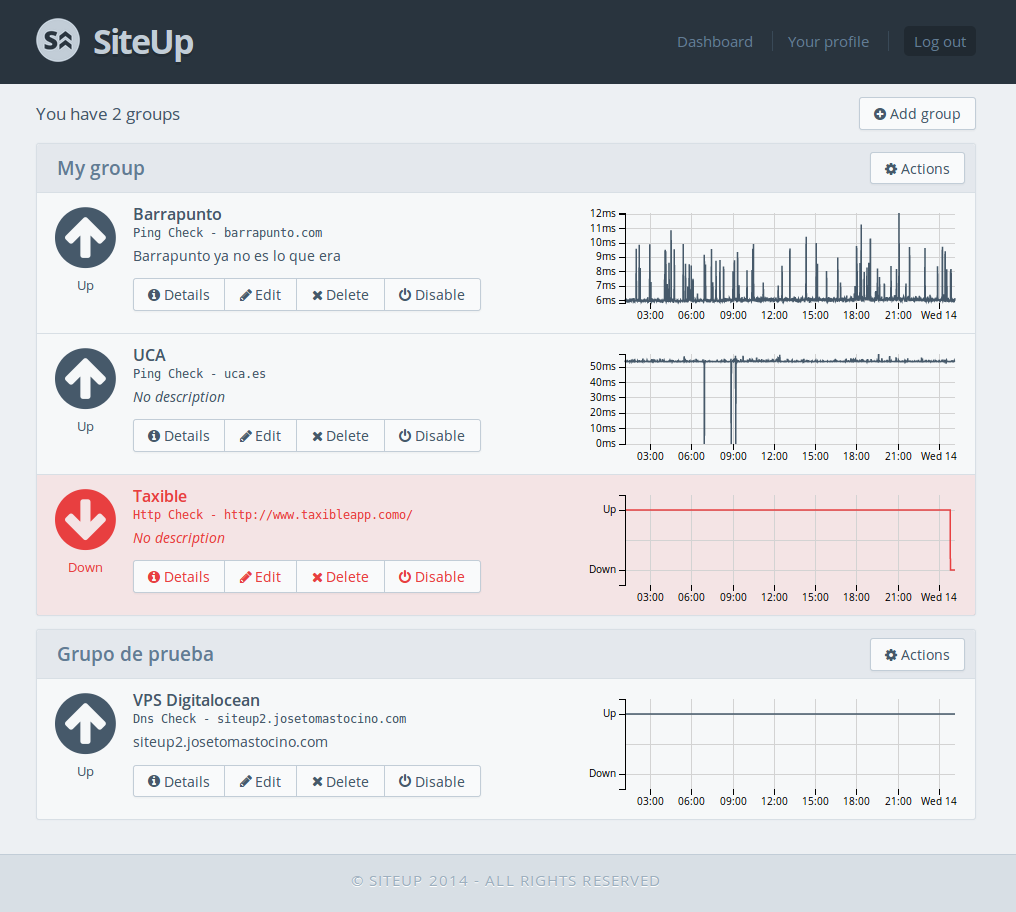
\includegraphics[width=0.7\textwidth]{detalle_dashboard}
  \caption{Detalle del panel principal de la plataforma web}
  \label{fig:detalle_dashboard}
\end{figure}

\subsection{Plataforma web}

El principal producto de SiteUp es la plataforma web de vigilancia, cuya
pantalla principal puede verse en la figura~\ref{fig:detalle_dashboard}. Ofrece
numerosas funcionalidades para los usuarios, previo registro en la aplicación en
línea, a través de los \textbf{chequeos}, los elementos principales de la
aplicación.

Se trata de puntos de vigilancia de cuatro tipos distintos que permiten
monitorizar multitud de aspectos distintos de un servicio en la web. A
continuación se describen cada uno de los tipos de chequeo incluidos en el
sistema.

\begin{figure}[t]
  \centering
  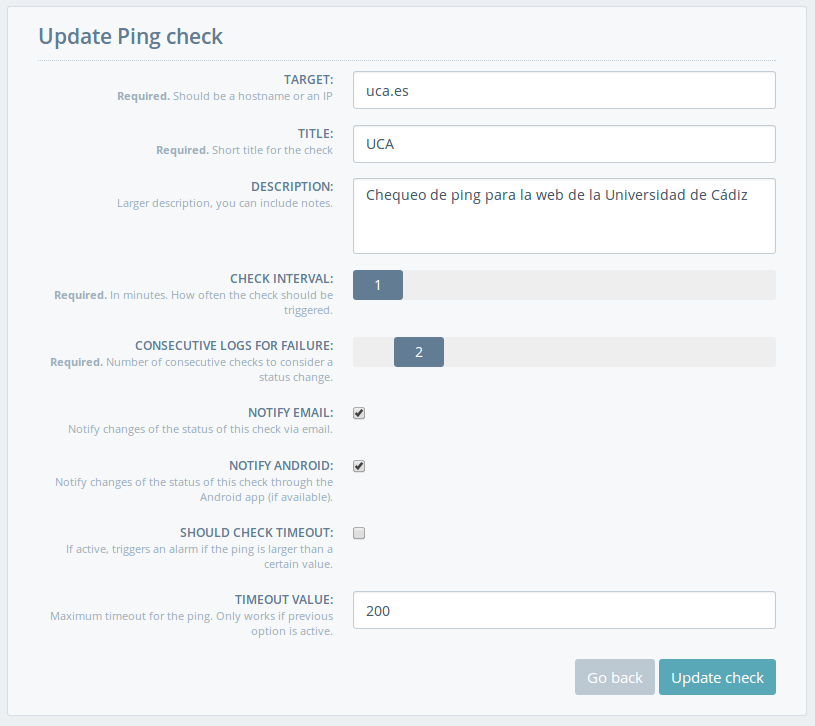
\includegraphics[width=0.7\textwidth]{detalle_formulario_chequeo}
  \caption{Formulario de edición de un chequeo}
  \label{fig:formulario_detalle_chequeo}
\end{figure}

\begin{itemize}

\item Chequeos de \textbf{tipo Ping}, que permiten saber si un \textit{host}
  remoto se encuentra en línea y si es capaz de responder en un tiempo
  establecido. \textbf{SiteUp} ofrece la posibilidad de verificar si un host
  responde a un chequeo de tipo Ping, opcionalmente verificando que la respuesta
  se obtiene dentro de un intervalo de tiempo establecido.

\item Chequeos mediante \textbf{peticiones HTTP} para verificar el correcto
  funcionamiento de un servidor web. \textbf{SiteUp} puede lanzar estos chequeos,
  pudiendo verificar tanto el código de estado obtenido como el propio cuerpo de
  la respuesta, por ejemplo cerciorándose de que una cierta cadena se encuentre
  dentro del contenido obtenido.

\item Chequeos de \textbf{puertos remotos}, que comprueban que un \textit{host}
  tiene accesible ciertos puertos asociados un servicio.  \textbf{SiteUp}
  permite crear chequeos de puertos remotos, informando de si estos puertos
  están abiertos o no, y opcionalmente dando la posibilidad de verificar que las
  conexiones entrantes reciben una respuesta adecuada por parte del servidor --
  una cadena preestablecida o \textit{mensaje de bienvenida}.

\item Chequeos de \textbf{registros DNS}, que permiten obtener información sobre
  un dominio o subdominio particular, verificando que el contenido de los
  registros es el correcto y no hay anomalías. \textbf{SiteUp} ofrece chequeos
  de registros DNS de cinco tipos distintos: \textbf{A}, \textbf{AAAA},
  \textbf{CNAME}, \textbf{MX} y \textbf{TXT}, siendo el más habitual el chequeo
  de registros tipo A, que comprueban que un dominio esté asociado a la IP
  apropiada -- esto es, que un dominio esté apuntando a un servidor correcto.

\end{itemize}



En \textbf{SiteUp}, el usuario puede crear chequeos de los tipos mencionados,
indicando los datos a través de un formulario como el de la
figura~\ref{fig:formulario_detalle_chequeo}. Entre los datos a incluir se
encuentra el \textbf{intervalo de chequeo}, que expresa la frecuencia a la que
debe ejecutarse el chequeo. Lo más habitual es utilizar un intervalo de un
minuto (el mínimo disponible), de forma que el chequeo se ejecute lo más
frecuentemente posible.

Otra propiedad importante es la \textbf{sensibilidad}. Este valor permite al
usuario establecer el número de comprobaciones necesarias para que el sistema
considere que un chequeo está en un estado de error. Esto es útil, por ejemplo,
al tratar con servidores que, a veces, dejan de responder momentáneamente sin
llegar a estar fuera de línea. En esos casos se pone un nivel de sensibilidad de
varios chequeos, de forma que el motor de \textbf{SiteUp} sólo se considere un
estado de error si el sistema detecta que la máquina remota ha fallado varias
veces consecutivas.

Los chequeos pueden \textbf{activarse o desactivarse} de forma temporal. Esto es
útil en situaciones en las que sea necesario hacer cambios en los detalles del
chequeo o en el servicio remoto y no queremos que se lancen las verificaciones
durante un intervalo de tiempo concreto. 

Es posible, además, hacer que el sistema envíe \textbf{notificaciones} cuando se
detecte un cambio de estado de un chequeo. Cada chequeo tiene dos opciones: una
para activar la notificación mediante correo electrónico y otra para la
notificación mediante la aplicación Android.

Por último, una vez que un chequeo se ha creado adecuadamente y está siendo
ejecutado por la plataforma, \textbf{SiteUp} ofrece una \textbf{pantalla de
  detalle} con gráficas detalladas del estado del chequeo para las últimas 24
horas, para la última semana y el último mes, con un informe detallado de los
cambios de estado detectados. La figura~\ref{fig:detalle_chequeo} muestra una
captura de la pantalla de detalle de un chequeo.

\subsubsection{Otras funcionalidades}

En la plataforma web, el usuario puede crear \textbf{grupos de chequeos} con los
que gestionar los chequeos de forma más sencilla, siendo posible activar,
desactivar o borrar los chequeos dentro de un grupo de forma masiva.

Además, el usuario tiene la posibilidad activar o desactivar el envío de un
\textbf{resumen diario} sobre sus chequeos, en el que se informa del estado de
cada chequeo, el tiempo que lleva en ese estado, el grupo al que pertenece,
etcétera.

La plataforma web está perfectamente adaptada para su acceso y uso desde
dispositivos móviles, ya sean teléfonos, tabletas, etc.

\begin{figure}[h]
  \centering
  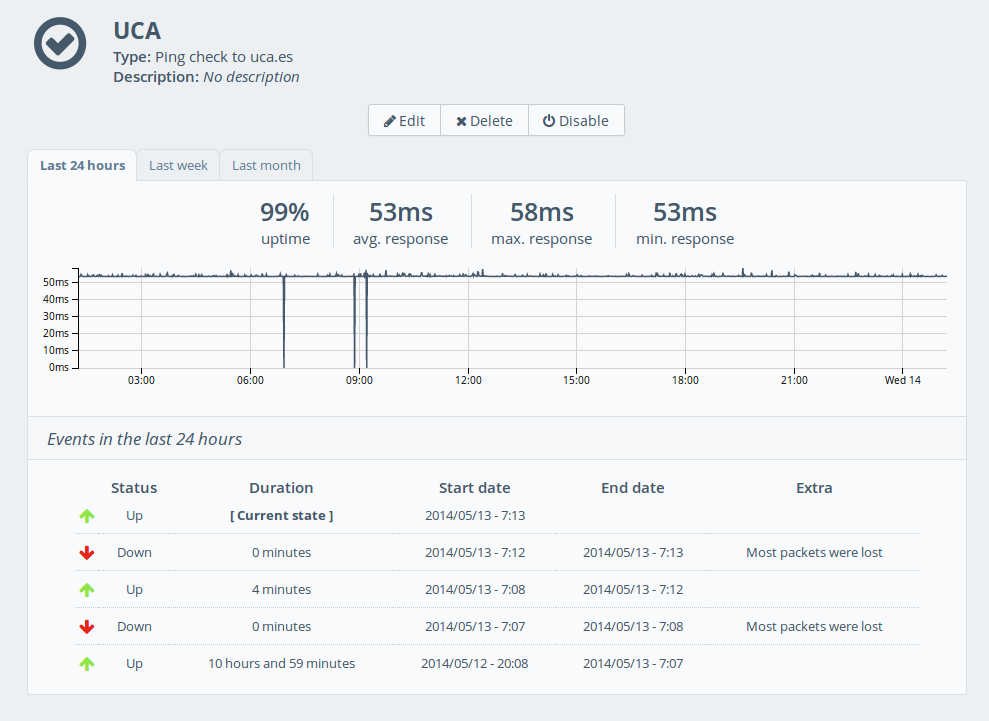
\includegraphics[width=0.7\textwidth]{detalle_chequeo}
  \caption{Detalle de un chequeo}
  \label{fig:detalle_chequeo}
\end{figure}

\subsection{Cliente móvil para Android}

\begin{figure}[hbt]
  \centering
  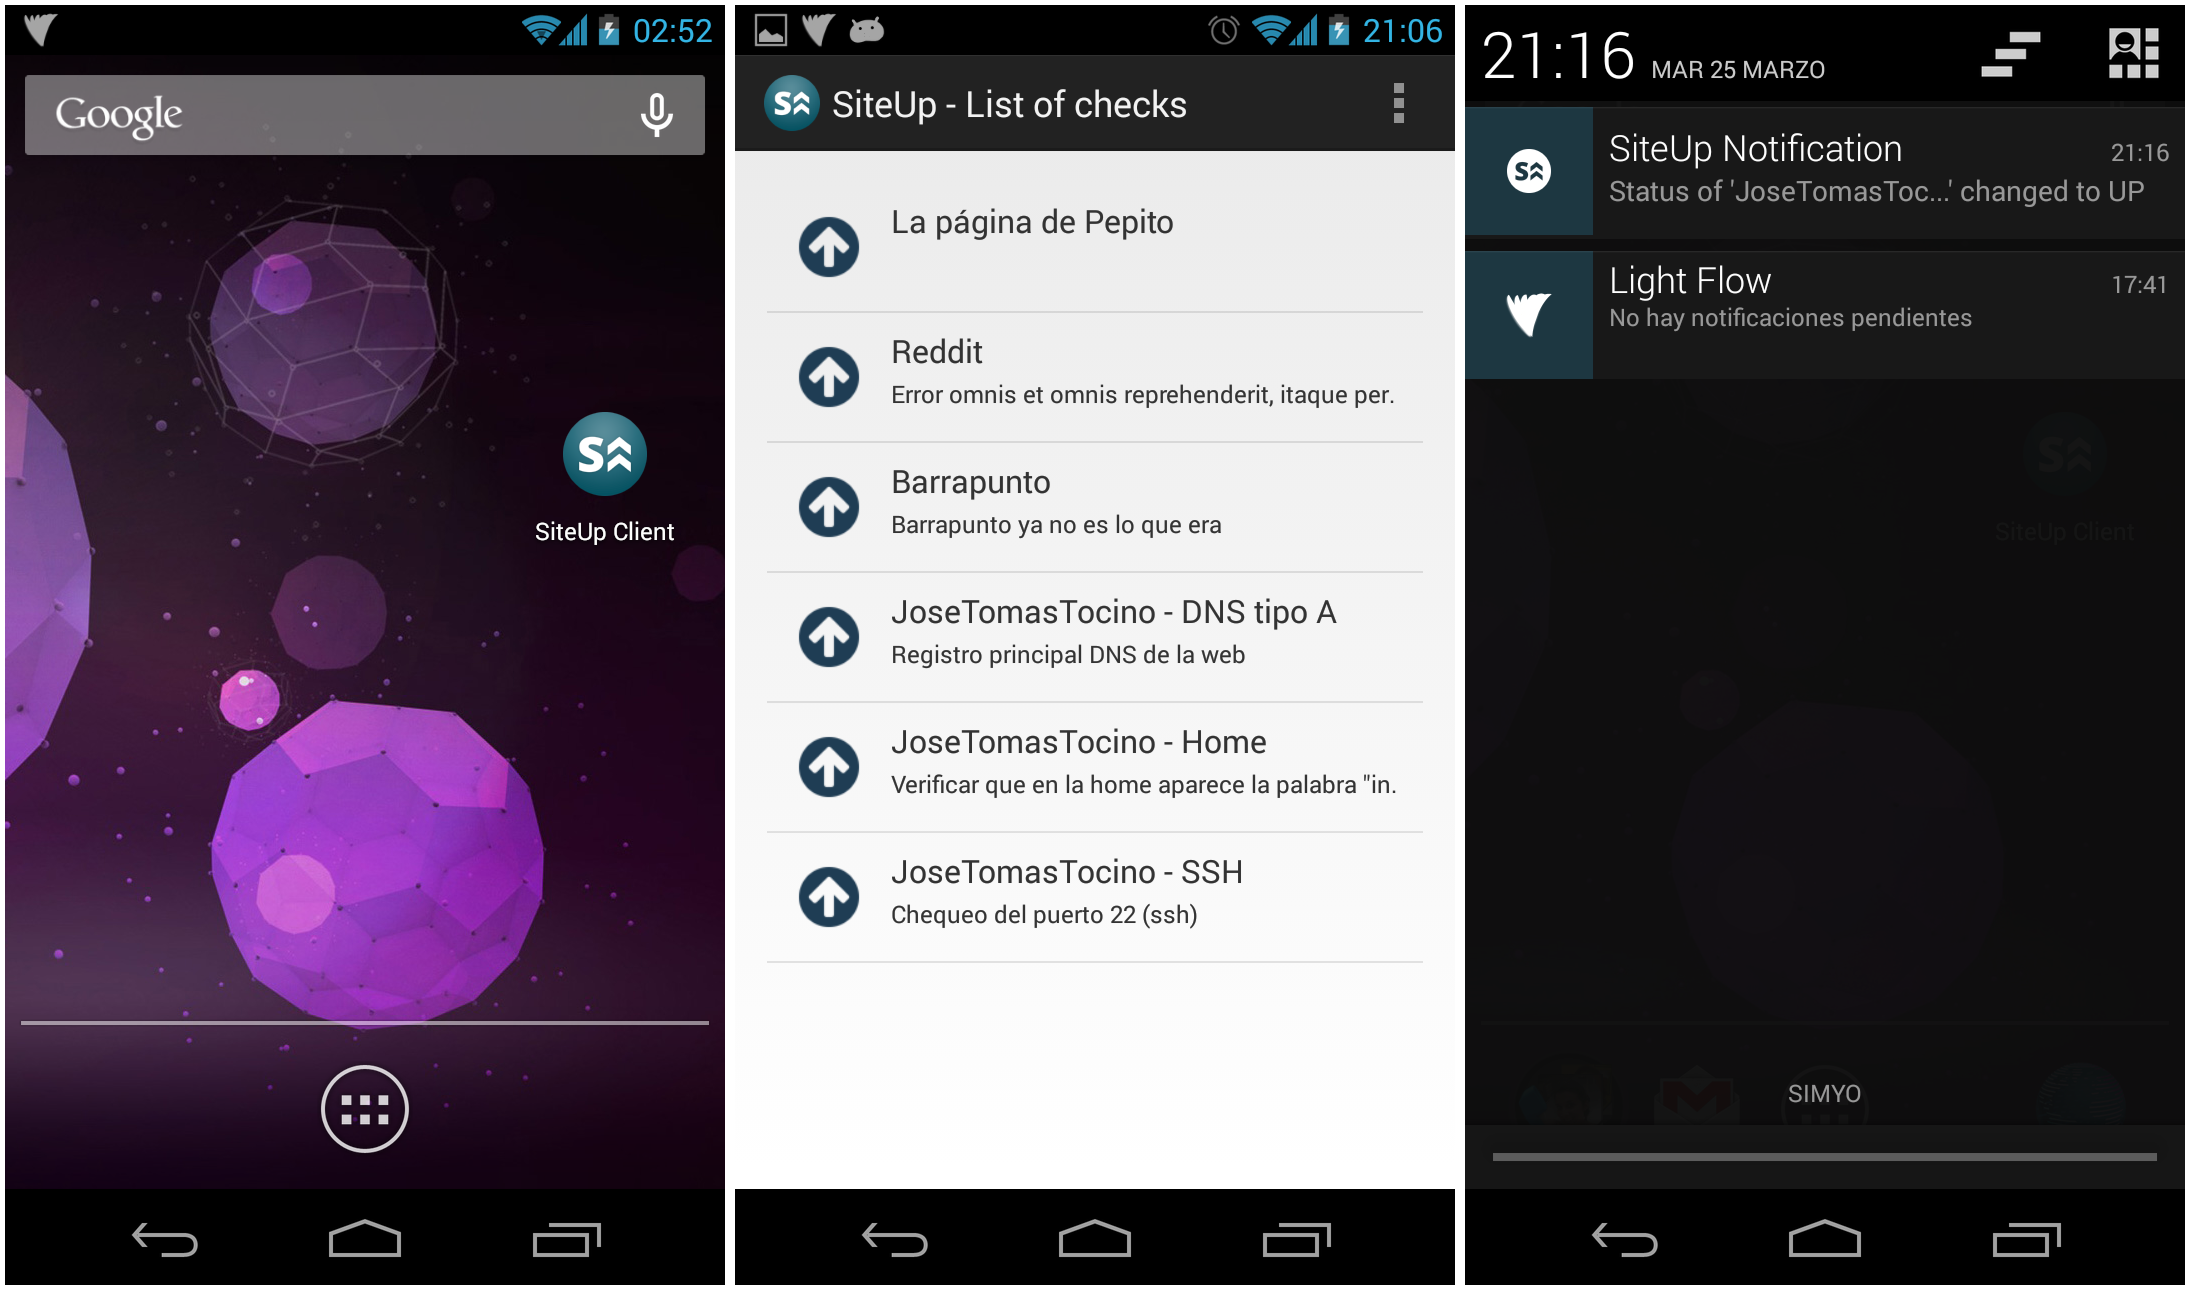
\includegraphics[width=0.85\textwidth]{capturas_android}
  \caption{Capturas del cliente SiteUp para Android}
  \label{fig:cliente_android}
\end{figure}

El segundo producto dentro del proyecto es \textbf{SiteUp Client}, una
aplicación nativa para el sistema operativo móvil Android que ofrece a los
usuarios dos funcionalidades principales.

En primer lugar, permite a los usuarios tener una \textbf{vista general} del
estado de los chequeos, viendo un listado de todos ellos así como su estado
actual. Desde esa vista general el usuario podrá pulsar en el chequeo que le
interese verificar, y será redirigido automáticamente a la página de detalle en
la plataforma web.

En segundo lugar y más importante, dispone de un \textbf{servicio de
  notificaciones} tipo \textit{Push} con las que la plataforma web podrá
notificar a los usuarios de manera instantánea. Los usuarios podrán recibir
notificaciones en cualquier momento mediante el sistema propio de la plataforma
Android, en la conocida como \textit{bandeja de notificaciones}. Éstas serán
fácilmente identificables gracias al uso del logotipo de \textbf{SiteUp} y el
texto informativo.

En la figura~\ref{fig:cliente_android} se pueden observar algunas capturas del
cliente para Android. 

% \FloatBarrier

\section{Desarrollo del sistema}

\begin{figure}[htbp]
  \centering
  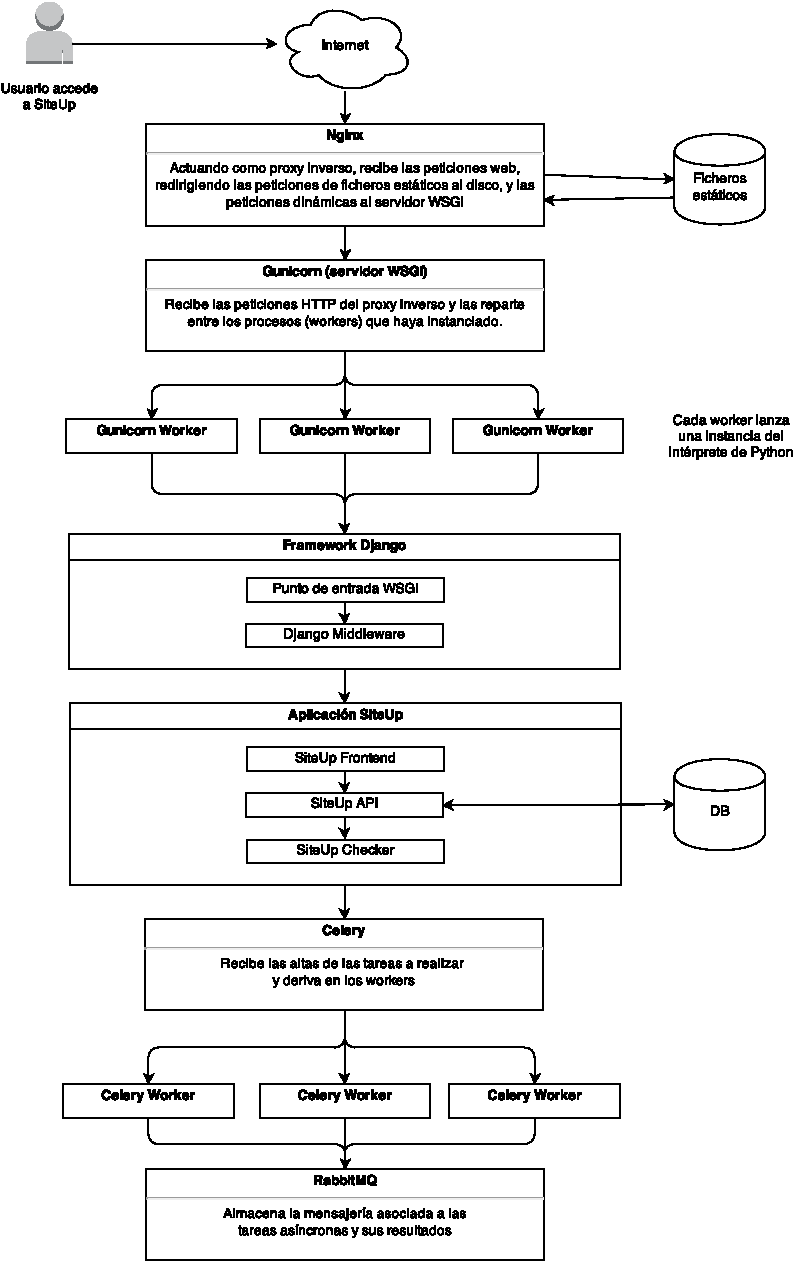
\includegraphics[width=0.9\textwidth]{diagrama_arquitectura_logica}
  \caption{Arquitectura lógica del sistema web}
  \label{fig:arquitectura-logica}
\end{figure}

El desarrollo de la plataforma web de \textbf{SiteUp} supuso un reto por el
cúmulo de tecnologías involucradas y las cuestiones que surgieron durante la
implementación. El \textit{stack} tecnológico utilizado y su integración con
SiteUp, esquematizados en la figura~\ref{fig:arquitectura-logica}, se detallan a
continuación:

\begin{itemize}
\item Como servidor frontal actuando de proxy inverso se ha utilizado
  \textbf{Nginx}~\cite{nginx}, encargado de, en primer lugar, dirigir las peticiones de
  recursos dinámicos al servidor de aplicaciones y, en segundo lugar, servir los
  ficheros estáticos de la aplicación.

\item El servidor de aplicaciones utilizado, \textbf{Gunicorn}~\cite{gunicorn},
  se encarga de recibir las peticiones HTTP dinámicas y repartirlas entre sus
  procesos (\textit{workers}), que se encargan de ejecutar el código Python.

\item El framework web sobre el que se ha desarrollado la aplicación,
  \textbf{Django}~\cite{django}, tiene múltiples responsabilidades. Entre las
  principales se encuentra la de determinar qué parte de la aplicación
  \textbf{SiteUp} ha de ejecutarse según la URL recibida, pasando la
  responsabilidad al código del proyecto.

\item El módulo frontal de la aplicación, \texttt{siteup\_frontend}, es el
  encargado de aceptar peticiones del usuario, recibiendo los datos de
  formularios y demás puntos de entrada, y devolviendo una respuesta
  adecuada. También se encarga de transmitir los mensajes apropiados al resto de
  modulos del proyecto. Por ejemplo, cuando un usuario da de alta un chequeo, se
  comunica con el módulo \texttt{siteup\_api}, encargado de la gestión del alta
  y mantenimiento de los datos de los chequeos en la base de datos. 

\item Una vez dados de alta los chequeos, el gestor de tareas
  \textbf{Celery}~\cite{celery} se encarga de listar y lanzar, de forma
  periódica, los chequeos que deban ejecutarse. Para ello, emite unas
  \textit{tareas} que son ejecutadas asíncronamente. El código para realizar los
  chequeos se encuentra modularizado dentro del paquete
  \texttt{siteup\_checker}, parte de \textbf{SiteUp}. Según el resultado de cada
  chequeo, este mismo módulo se encarga de enviar notificaciones mediante correo
  electrónico o a la aplicación Android mediante el servicio \textbf{Google
    Cloud Messaging}~\cite{gcm}.

\end{itemize}

Además de las mencionadas, se han utilizado muchas otras tecnologías y
herramientas de apoyo al desarrollo, que se detallan más profundamente en la
memoria del proyecto.

\subsection{Detalle de implementación del chequeo por ping}

Uno de los primeros retos que se encontraron en la etapa de desarrollo fue la
ejecución de chequeos por ping. Para poder enviar paquetes en el protocolo ICMP
es necesario tener permisos de administrador (o \textit{root}) en el sistema,
cosa que no es habitual al ejecutar una aplicación web. Este requisito se da
porque es necesario abrir un socket puro (\textit{raw socket}), un tipo especial
de socket que solo se usa en ocasiones especiales y cuya creación se restringe
al administrador del sistema~\cite{linux_man_capabilities}.

La alternativa más habitual es ejecutar el comando \textbf{\texttt{ping}} de
forma externa, y procesar su salida. El comando \texttt{ping} tiene un permiso
de acceso especial que permite a cualquier usuario lanzar el ejecutable emulando
temporalmente los privilegios del usuario \texttt{root}.

Para procesar la salida del comando se utilizó una \textbf{expresión regular} de
gran envergadura, que tenía en cuenta casos especiales como aquellos en los que
los paquetes ICMP se perdiesen. Se presenta a continuación un fragmento del
código involucrado.

\begin{pythoncode}
process = subprocess.Popen(["ping", "-c3", "-w2", target], 
                           stdout=subprocess.PIPE, 
                           stderr=subprocess.PIPE)
# Get the output
ping_raw_response, ping_raw_error = process.communicate()

# Compile regular expression to parse ping's output
matcher = re.compile(r"""
^PING \s+                            # Header
(?P<host>.*?) \s+                    # Host
\((?P<ip>.*?)\)                      # IP address
.*?                                  # Ignore individual pings
(?P<transmitted>\d+) \s+ packets       .*?       # Packets transmitted
(?P<received>\d+) \s+ received         .*?       # Packets received
ms                                     \s*       # Ending of the statistics line
(                                    # Non-capturing group for the stats
rtt .* = \s+                         # Separator
(?P<min>[^/]*)/                      # Min time
(?P<avg>[^/]*)/                      # Avg time
(?P<max>[^/]*)/                      # Max time
(?P<mdev>.*?) \s ms                  # Mdev
)?

""", re.DOTALL | re.IGNORECASE | re.MULTILINE | re.VERBOSE)

# Run the regular expression to parse ping's output
results = matcher.match(ping_raw_response)
\end{pythoncode}

\subsection{Verificación y pruebas}

Para comprobar la correcta ejecución del software se han llevado a cabo varios
procesos de verificación y baterías de pruebas a distintos niveles, tanto de
manera autónoma como manualmente.

\subsubsection{Pruebas funcionales}

Se ha llevado a cabo un gran número de pruebas funcionales, que tratan de
comprobar el correcto funcionamiento de las funciones del
software. Principalmente se han realizado \textbf{pruebas unitarias} y
\textbf{de integración} haciendo uso de las capacidades de testing que provee el
framework de Django, apoyándose a la vez en servicios de terceros para
comprobar, por ejemplo, el correcto funcionamiento de las conexiones HTTP.

Por otro lado, se fueron lanzando \textbf{pruebas de sistema} durante cada una
de las iteraciones del desarrollo, utilizando un entorno virtual con un servidor
de pruebas y software de \textit{throttling} de red para simular condiciones de
red adversas que se asemejasen a entornos reales.

Finalmente, se utilizó un servidor real, ubicado en Alemania, en el que se
desplegó el producto para llevar a cabo \textbf{pruebas de aceptación}. El
servidor ha permanecido online desde mediados del mes de febrero hasta la fecha,
recibiendo las actualizaciones del software según se iba desarrollando y
funcionando de manera regular.

\subsubsection{Pruebas no funcionales}

Con objeto de verificar aspectos del proyecto más allá de su funcionalidad, las
pruebas no funcionales cubrieron bastantes frentes distintos. En particular:

\begin{itemize}
\item Se llevaron a cabo pruebas de \textbf{seguridad}, centradas principalmente
  en verificar que la información de los usuarios y las áreas privadas del sitio
  web eran seguras.

\item Las pruebas de \textbf{fiabilidad} verificaron que la disponibilidad del
  servicio era la correcta y que los chequeos se lanzaban dentro de un margen de
  tiempo apropiado.

\item Mediante pruebas de \textbf{accesibilidad} se comprobó que la plataforma
  web era accesible desde cualquier clase de dispositivo móvil con acceso a
  internet. Así, se llegó a probar la funcionalidad desde más de 8 dispositivos
  distintos, obteniendo resultados favorables en todos los casos.

\end{itemize}

\subsubsection{Verificación de la calidad del código}

En la medida de lo posible se ha seguido la guía de estilo oficial de Python,
expuesta en el documento oficial PEP8~\cite{pep8} por el propio creador del
lenguaje, Guido van Rossum. Para reforzar el seguimiento de estas buenas
prácticas de código se ha hecho uso de herramientas de verificación automática,
que comprueban que el código se ajuste a las convenciones de nombrado, sintaxis
y otras recomendaciones presentes en el citado documento.


\section{Conclusiones y difusión}

Durante el transcurso del desarrollo de SiteUp, y sobre todo al término del
mismo, se han obtenido unas conclusiones y unos resultados, tanto de forma
personal como para con la comunidad, que se reflejan a continuación.

\subsection{Objetivos cumplidos}
Al término del desarrollo del proyecto, el proyecto ha completado todos los
objetivos a cumplir. En particular:

\begin{itemize}
\item Se ha creado un conjunto de herramientas de chequeo de servicios de
  Internet, que se encuentra disponible en el módulo
  \texttt{siteup\_checker/monitoring} del proyecto.
\item Se ha creado una aplicación online de acceso público con la que los
  usuarios pueden gestionar sus chequeos de manera sencilla, que en la fecha de
  escritura de la presente memoria es accesible en la url
  \url{http://siteup.josetomastocino.com}.
\item Se ha establecido un sistema de notificaciones con el que mantener
  informados a los usuarios tanto por correo electrónico como mediante una
  aplicación móvil para el sistema operativo Android desarrollada a tal
  efecto. Actualmente la aplicación se encuentra disponible en la forja de
  código~\cite{forja} y en un futuro lo estará en el Google Play Store.


% \item Investigar y conocer los vectores de vigilancia usados habitualmente para
%   monitorizar servicios de Internet.
% \item Ampliar mis conocimientos sobre desarrollo web en general y las
%   tecnologías de \textit{back-end} en particular.
% \item Adquirir soltura en el uso del lenguaje de programación Python en entornos
%   web.
% \item Obtener una base de conocimientos sobre el desarrollo de aplicaciones
%   sobre la plataforma móvil Android.
% \item Utilizar un enfoque de análisis, diseño y codificación orientado
%   a objetos, de una forma lo más clara y modular posible, para
%   permitir ampliaciones y modificaciones sobre la aplicación por
%   terceras personas.
% \item Hacer uso de herramientas básicas en el desarrollo de software,
%   como son los sistemas de control de versiones para llevar
%   un control realista del desarrollo del software, así como hacer de
%   las veces de sistema de copias de seguridad.

\end{itemize}

La compleción total de los objetivos funcionales también pone de manifiesto que
se han alcanzado satisfactoriamente los objetivos transversales y personales
que se presentaron. Se han afianzado fuertemente los conocimientos de
desarrollo web en general y con Django en particular hasta un nivel de
competencia suficiente para servir como baza en la búsqueda laboral. Además,
SiteUp ha servido satisfactoriamente como primera incursión en el mundo del
desarrollo de aplicaciones Android.

\subsection{Conclusiones personales}

SiteUp es un proyecto personal que ha surgido para suplir una \textbf{necesidad}
real y específica y que, al término del desarrollo, ha conseguido su
objetivo. La idea inicial ha servido como eje motor del proyecto en todo
momento. Si se diese la situación presentada en el inicio, el proyecto SiteUp
sería capaz de detectar el problema e informar en consecuencia.


\subsubsection{Lecciones aprendidas}

La cantidad de \textbf{tecnologías} diferentes utilizadas en cada uno de los
niveles de abstracción del proyecto es bastante grande. Adquirir una competencia
básica en todas estas tecnologías ha sido una tarea de una envergadura
importante, y la correcta ejecución del sistema es comparable al mecanismo de un
reloj, en el que todas las piezas deben funcionar de manera coordinada.

Desde la configuración de los numerosos servicios usados en el entorno de
producción, al despliegue de la aplicación, pasando por el desarrollo de los
módulos de chequeo, hasta llegar a la implementación del código de la capa de
presentación, sin olvidar la implementación de la aplicación Android. En todos
los niveles, en unos en mayor medida que en otros, se ha alcanzado una soltura
suficiente para el desarrollo y posterior lanzamiento de un producto completo.

Al tratarse de un proyecto de ejecución continua en el que constantemente se
están haciendo chequeos y enviando notificaciones, el flujo de \textit{feedback}
entre los usuarios y el desarrollador (que en las etapas iniciales son la misma
persona) es mucho más \textbf{dinámico} que en cualquier otro proyecto en el que
la ejecución fuese momentánea, como un juego o una aplicación de
escritorio. Este planteamiento ha permitido que en SiteUp se hayan detectado
rápidamente conflictos y problemas en el sitio, como por ejemplo que algunos
usuarios prefieren no recibir resúmenes diarios de sus chequeos, motivando la
inclusión de una opción en sus perfiles para desactivar esta funcionalidad.

\subsection{Difusión y reconocimiento}

Finalmente, gracias a SiteUp tuve la oportunidad de participar en el \textit{VIII Concurso
  Universitario de Software Libre}~\cite{cusl}, pudiendo presentar el proyecto a
la comunidad universitaria local el miércoles 23 de abril de 2014 en la
Universidad de Cádiz. En la presentación obtuve opiniones y consejos para
mejorar en el proyecto que en mayor o menor medida se han acabado tomando en
cuenta e integrando.

El jurado del premio local decidió nombrar a SiteUp ganador del premio al
\textit{Mejor Proyecto Innovador de Software Libre}~\cite{cusl-local}.


\bibliographystyle{hispa-annote}
\bibliography{bibliografia}

\vspace{0.75cm}

\begin{center}
{\footnotesize Este documento se halla bajo la licencia FDL de GNU (Free Documentation
  License)\\ \url{http://www.gnu.org/licenses/fdl.html} }   
\end{center}

\end{document}
